\documentclass[review]{elsarticle}

\usepackage{lineno,hyperref}
\modulolinenumbers[5]

\usepackage{adjustbox}
\usepackage{amsmath}
\DeclareMathOperator*{\argmax}{arg\,max}
\DeclareMathOperator*{\argmin}{arg\,min}
%\usepackage{algorithmic}
%\usepackage{algorithm}
\usepackage{algorithm,algpseudocode,float}

\algnewcommand\algorithmicforeach{\textbf{for each}}
\algdef{S}[FOR]{ForEach}[1]{\algorithmicforeach\ #1\ \algorithmicdo}

\journal{Journal of Parallel and Distributed Computing}

%%%%%%%%%%%%%%%%%%%%%%%
%% Elsevier bibliography styles
%%%%%%%%%%%%%%%%%%%%%%%
%% To change the style, put a % in front of the second line of the current style and
%% remove the % from the second line of the style you would like to use.
%%%%%%%%%%%%%%%%%%%%%%%

%% Numbered
%\bibliographystyle{model1-num-names}

%% Numbered without titles
%\bibliographystyle{model1a-num-names}

%% Harvard
%\bibliographystyle{model2-names.bst}\biboptions{authoryear}

%% Vancouver numbered
%\usepackage{numcompress}\bibliographystyle{model3-num-names}

%% Vancouver name/year
%\usepackage{numcompress}\bibliographystyle{model4-names}\biboptions{authoryear}

%% APA style
%\bibliographystyle{model5-names}\biboptions{authoryear}

%% AMA style
%\usepackage{numcompress}\bibliographystyle{model6-num-names}

%% `Elsevier LaTeX' style
\bibliographystyle{elsarticle-num}
%%%%%%%%%%%%%%%%%%%%%%%

\begin{document}

\begin{frontmatter}

\title{Parallel Solving of Multiple Information-Coordinated Global Optimization Problems}

%% Group authors per affiliation:
%\author{Victor Gergel \and Evgeniy Kozinov}
%\address{Lobachevsky State University of Nizhni Novgorod, Nizhni Novgorod, Russia}
%\ead{gergel@unn.ru}

\author[mymainaddress]{Victor Gergel}
\ead{gergel@unn.ru}

\author[mymainaddress]{Evgeniy Kozinov}
\ead{evgeny.kozinov@itmm.unn.ru}

\address[mymainaddress]{Institute of Informational Technologies, Mathematics and Mechanics, Mathematical Center, Lobachevsky State University of Nizhny Novgorod, Nizhni Novgorod, Russia}



\begin{abstract}
This paper proposes an efficient approach for the parallel solution of computationally time consuming problems of multiple global optimization, in which minimized functions can be multiextremal and calculating function values may require huge amounts of computations. The proposed approach is based on the information-statistical theory of global optimization, within which a general computational scheme of global optimization methods is proposed. In the paper, this general scheme is expanded by the possible reuse of search information obtained in the process of computations when solving multiple global optimization problems. Within the framework of the proposed generalized scheme, parallel algorithms are proposed for computational systems with shared and distributed memory. Results of computational experiments demonstrated that the proposed approach can significantly reduce the computational complexity of solving multiple global optimization problems.
\end{abstract}

\begin{keyword}
Global optimization \sep dimensionality reduction \sep search information \sep parallel methods of global search \sep computational complexity.
\end{keyword}

\end{frontmatter}

\linenumbers


\section{Introduction}\label{sec:1}


Since the early 1960s, the problems of global optimization (GO) have continued to be a grand challenge to the theory and practice of optimization. In contrast to local optimization problems, when searching for a global minimum, the numerical method must evaluate the behavior of the function to be optimized in the entire global search domain. In general, GO problems are subject to the ``dimensionality curse'', when the volume of computations performed increases exponentially with increasing dimensionality. Such computational complexity, as well as high practical demand, have led to a great deal of research activity in the field of global optimization. An overview of approaches developed for solving global optimization problems is presented, for example, in a number of recent monographs and reviews -- see \cite{c1,c2,c3,c4,c5,c6,c7,c8,c9}.

The first and obvious approach is to use local methods that allow one to efficiently solve optimization problems with unimodal objective functions \cite{c1}. In the case of multiextremal problems, local methods should be applied repeatedly to find global minima using different initial points. Research in this direction began as early as the 1960s and is still relevant today \cite{c10,c11,c12}. Unfortunately, the problem of choosing initial points still remains open -- even using a significant number of initial points does not guarantee a reliable solution of global optimization problems. Another obvious approach is to construct a grid in the search domain, at the nodes of which the values of functions to be minimized are computed \cite{c2,c3,c4,c5}. To reduce computational complexity of uniform grids, this approach envisages different methods for construction of non-uniform grids, which would be denser only in the vicinity of the global minimum. This line of research is developing in the field of so-called nature-inspired metaheuristic methods, including, for example, genetic algorithms, bee algorithms, particle swarm optimization, simulated annealing, ant colony optimization, and firefly algorithms, etc. \cite{c4,c13,c14,c15}. A large number of applied problems have been solved using these methods, however, as before, it is also difficult to obtain guaranteed estimates of the accuracy when finding globally-optimal solutions for these algorithms.

Yet another line of research in the field of global optimization is based on the assumption that the analytical form of the functions to be optimized is known. In this case, we can speak of d.c.(difference of convex) optimization problems in which nonconvex multiextremal functions are represented as a difference of two convex functions \cite{c16,c17}. Another approach to the development of global optimization methods in this area is based on the use of interval analysis methods \cite{c18}.

In case analytical expressions for the functions to be optimized are not known (and this is a typical situation for choosing the best solutions in applied optimization problems), it should be understood that numerical estimates of global optimal solutions cannot in principle be obtained if there are no a priori assumptions about the behaviour of the functions to be minimized. One if the most widely used ways for specifying such information is to assume the validity of the Lipschitz condition according to which possible changes of the function to be minimized are restricted by the variation values of the parameters being varied. The use of this assumption leads to a class of Lipschitzian global optimization problems that has been extensively explored \cite{c3,c6,c7,c19,c19,c20,c21,c22,c23}.  As a rule, algorithms for solving this class of problems are adaptive, i.e. when determining the points for global search iterations, algorithms tend to use all the search information obtained in the process of computation. Such adaptivity leads to non-uniform grids and makes it possible to construct estimates of the global minimum based on a finite number of global search iterations. A large number of results in this direction have been obtained within the framework of the rapidly developing information-statistical theory of global optimization \cite{c6}. It should also be noted that multivariate algorithms of this class quite often use dimensionality reduction using Peano curves or nested optimization scheme \cite{c23}. One can also mention the class of DIRECT-type methods using several estimates of the Lipschitz constant chosen from some set of possible values; a detailed review of this line of research is given in \cite{c22}.


The paper proposes a further complication in formulating the decision making problems, when not only one, but several global optimization problems need to be solved simultaneously. Such problems are encountered, for example, when one needs to find several efficient solutions of multicriteria optimization problems or when part of the variable parameters in the optimization problem can take only a certain number of discrete values. For the first time, the formulation of such multiple global optimization (MGO) was considered in \cite{c25,c26}, and then was investigated in \cite{c27,c28}. The relatively limited attention given to MGO problems is most likely due to the high computational complexity involved for solving even one GO problem.

In general, MGO problems can be solved by a simple sequential (or parallel) solution of individual problems from a set. However, this approach results in a many-fold increase in the computational complexity of solving such problems. Meanwhile, individual GO problems that are part of the same MGO problem may have a certain informational interrelation -- a similar connectivity is observed, for example, when methods based on scalarization of the vector efficiency criterion are applied to solve multicriteria optimization (MCO) problems. In this case, it becomes necessary to solve multiple scalar (in the general case, global) optimization problems in order to find several efficient decisions  for MCO problems -- see, for example, \cite{c29,c30,c31,c32,c33}. Such interconnectedness of GO problems can be used to reduce significantly the amount of computation performed when solving the entire set of problems.

The approach proposed in this paper assumes that the computational values of any function of the same MGO problem can be recalculated to the values of any other functions of the set without any time consuming calculations. In such cases, all the search information obtained in solving a particular problem can be used in solving all other problems in the set. Such repeated reuse of search information can significantly reduce the amount of computation performed, up to just a few iterations when solving the next GO problems. In addition, the presence of informational connectivity significantly expands the possibilities of a parallel solution for MGO problems. The paper proposes two new parallel computational schemes: a cooperative scheme, which means the search information is exchanged between computational devices with distributed memory used for solving several GO problems in parallel, and a competitive scheme, which occurs when GO problems solved in parallel compete with each other for the use of available computational resources with shared memory.

The structure of the paper is as follows. Section \ref{sec:2} sets out the problem of multiple global optimization. Section \ref{sec:3} presents a general computational scheme for solving global search problems. Section \ref{sec:4} proposes parallel methods for solving MGO problems by using computational systems with shared and distributed memory. Section \ref{sec:5} contains the results of numerical experiments confirming the effectiveness of the proposed parallel methods. In the conclusion, results are discussed and the main directions for further research are presented.

\section{Problem Statement}\label{sec:2}

The multiple global optimization (MGO) problem consists in solving a family of problems:
\begin{equation}\label{eq:1}
f_i(y^*) = \argmin f_i(y), y \in D, 1 \leq i \leq s,
\end{equation}

\begin{equation}\label{eq:2}
D  = \{ y\in R^N: a_i \leq y_i \leq b_i, 1 \leq i \leq N \}
\end{equation}
defined by a set of optimized functions
\begin{equation}\label{eq:3}
F(y) = \{ f_1(y),  f_2(y),\dots, f_s(y) \},
\end{equation}
where $y = (y_1,y_2,\dots,y_N)$ is the vector of varied parameters, $N$ is the dimension of the global optimization problems to be solved, and $D$ is the search domain for the given vectors $a$ and $b$. 

In this paper, it is assumed that the functions $f_i(y)$, $1 \leq i \leq s$, can be multiextremal, and the procedures for calculating the values of these functions at points in the search domain $y \in D$ can be computationally expensive. It is also assumed that the functions $f_i(y)$, $1 \leq i \leq s$, satisfy the Lipschitz condition
\begin{equation}\label{eq:4}
|f_i (y')-f_i (y'')| \leq L_i \|y'-y''\|, y',y''\in D, 1 \leq i \leq s,
\end{equation}
where $L_i$ is the Lipschitz constant for the function $f_i(y)$, $1 \leq i \leq s$, and ${\|*\|}$ denotes the Euclidean norm in $R^N$. Fulfillment of the Lipschitz condition allows us to construct numerical estimates of the possible behavior of minimized functions based on a finite set of calculated function values at points in the search domain.


A key condition of this approach is the assumption that any calculated value of any function $f_i(y)$, $1 \leq i \leq s$, of the set $F$ at an arbitrary point $y \in D$ of the search domain $D$ can be transformed to the value of any other function of the set $F$ at the same point $y \in D$ without any time consuming computations, in a time significantly shorter compared to the computation time values of the functions $f_i(y)$, $1 \leq i \leq s$. In other words, there must be a transformation $Z$ such that
\begin{equation}\label{eq:5}
\begin{matrix}
\forall 1 \leq i, j \leq s, \bar{y} \in D \Rightarrow z_i=Z(z_j ), z_i = f_i (\bar{y}),z_j=f_j (\bar{y}), \\
T(Z) \ll T(f_l (y) ),1 \leq l \leq s,
\end{matrix}
\end{equation}
where $T(*)$  is the computation time of the expression given in parenthesis.

This condition is fulfilled, for example, when solving multicriteria optimization (MCO) problems 
\begin{equation}\label{eq:6}
g(y) = (g_1(y), g_2(y), \dots , g_m(y)) \to min,  y\in D.
\end{equation}

To find efficient (unimprovable) solutions, a widely used approach is based on the reduction (scalarization) of the vector criterion $g(y)$ to the general scalar criterion, the minimization of which will lead to the Pareto optimal solution of the MCO problem \cite{c29,c30,c31,c32,c33}. So, when using minimax convolution, the vector criterion $g(y)$ from (\ref{eq:6}) reduces to the scalar criterion
\begin{equation}\label{eq:7}
\begin{matrix}
G(\lambda,y)=\max{(\lambda_l g_l(y),1 \leq l \leq m)},	\\
\lambda=(\lambda_1,\lambda_2,\dots,\lambda_m)\in \Lambda \subset R^m:\sum_{l=1}^m{\lambda_l =1},\lambda_l\geq 0,1 \leq l \leq m.
\end{matrix}
\end{equation}


If it is necessary to find several efficient decisions to the MCO problem (\ref{eq:6}), the optimization of the scalar criterion $G(\lambda,y)$ from (\ref{eq:7}) is performed for different values of the coefficients $\lambda \in \Lambda$. Thus, the problem of finding a set of efficient decisions for the MCO problem can be represented as a statement of the MGO problem (\ref{eq:1})-(\ref{eq:3}), where the optimized functions $f_i(y)$, $1 \leq i \leq s$, and the set $F$ are defined as
\begin{equation}\label{eq:8}
F(y)= \{ G(\lambda_i,y),1 \leq l \leq s\}.
\end{equation}

As a result, if the values of efficiency criteria $g_i(y)$, $1 \leq i \leq m$, are computed at some point $y=\bar{y}$ of the search domain $D$, then the value of the scalar criterion $G(\lambda,y)$ can be computed at the point $\bar{y} \in D$ for any values of the coefficients $\lambda \in \Lambda$. In this case the transformation of $Z$ from (\ref{eq:5}) is determined by the expression (\ref{eq:7}) at fixed values of the criteria $g_l (y)$,$1 \leq l \leq m$) \cite{c27,c28}.

The ability to quickly convert the calculated values of optimized functions determines the need to accumulate and use search information obtained in the calculation process
\begin{equation}\label{eq:9}
\omega_k (j)=\{(y^i,f^i=f_j(y^i)):1 \leq i \leq k \},1 \leq j \leq s,
\end{equation}
where $j$, $1 \leq j \leq s$, is the number of the current function being minimized $f_j (y)$ of the set $F$ from (\ref{eq:3}), $k$ is the number of iterations of the global search, $y^i \in D$, $1 \leq i \leq k$,  are points in which the values of the optimized problems of the set $F$ were computed, and $f^i$, $1 \leq i \leq k$, are the values of the function $f_j (y)$ at these points (the procedure for calculating the value of the function will be called a trial). Global optimization methods can use this search information, thereby ensuring the ability to solve each successive problem of the set $F$, taking into account the results of all previous calculations. Numerical experiments that were performed (see Section \ref{sec:5}), confirm that such repeated use of search information reduces the number of iterations of the global search required to solve the next problem of the set $F$ (even to the point of performing just a few search iterations).

In conclusion, it should be noted that, in general, the set of functions being minimized $F$ from (\ref{eq:3}) can be formed dynamically in the course of calculations by adding new or removing existing global optimization functions
\begin{equation}\label{eq:10}
F'=F+(-) f(y).
\end{equation}


\section{A General Computational Scheme for Solving Global Optimization Problems}\label{sec:3}

The approach proposed in this paper is based on two key ideas used in the framework of the information-statistical theory of global optimization \cite{c6}.

In accordance with this theory, first of all, dimensionality reduction is achieved using the Peano space-filling curves (evolvents) $y(x)$, uniquely and continuously mapping the interval [0,1] to the $N$-dimensional domain $D$ -- see, for example, \cite{c6,c23}. As a result of this reduction, multidimensional global optimization problems (\ref{eq:1})-(\ref{eq:3}) can be reduced to one-dimensional ones:

\begin{equation}\label{eq:11}
\min {f_i (y(x))} = \min{f_i (y)}, x \in [0,1], y \in D, 1 \leq i \leq s.
\end{equation}

It should be noted that the one-dimensional functions obtained as a result of the reduction satisfy the uniform H\"older condition, i.e.
\begin{equation}\label{eq:12}
|f_i (y(x'))-f_i (y(x''))| \leq H_i |x'-x''|^{1/N}, x',x''\in [0,1], 1 \leq i \leq s,
\end{equation}
where the constants $H_i$ are determined by the relation $H_i = 2L_i \sqrt{N+3}$, ${1 \leq i \leq s}$, $L_i$ are the Lipschitz constants from (\ref{eq:4}), and $N$ is the dimensionality of the optimization problem (\ref{eq:1}).

Dimensionality reduction significantly decreases the computational complexity of analyzing multidimensional data to highlight the subdomains of the search domain $D$ for the efficient continuation of the global search, and reduces the severity of the ``curse of dimensionality'' problem in solving multidimensional optimization problems. After dimensionality reduction, the search information $\omega_k$ from (\ref{eq:9}) takes the form
\begin{equation}\label{eq:13}
A_k (j)=\{ (x_i, y(x_i), z_i=f_j (y(x_i) ): 1 \leq i \leq k \}, 1 \leq j \leq s,
\end{equation}
in which, in addition to the reduced representation, the data is arranged in the ascending order\footnote{Data ordering is reflected by using a subscript.} of points $x_i$,  $1 \leq i \leq k$, i.e.

\begin{equation}\label{eq:14}
x_1< x_2< \cdots < x_k
\end{equation}
for a more efficient execution of global search algorithms. It should be noted that in optimizing the reduced one-dimensional functions $f_i (y(x))$, $1 \leq i \leq s$, many one-dimensional global search algorithms can be used (possibly after some generalization).

Numerical methods for constructing approximations of Peano space-filling curves (evolvents) with a given accuracy for a given dimensionality are considered in \cite{c6}; examples of such approximations are shown in Fig.\ref{fig:1}.

Further, in the framework of information-statistical theory, a general computational scheme of global optimization algorithms is proposed \cite{c6}. This scheme can be summarized as follows.

\begin{figure}
  \centering
  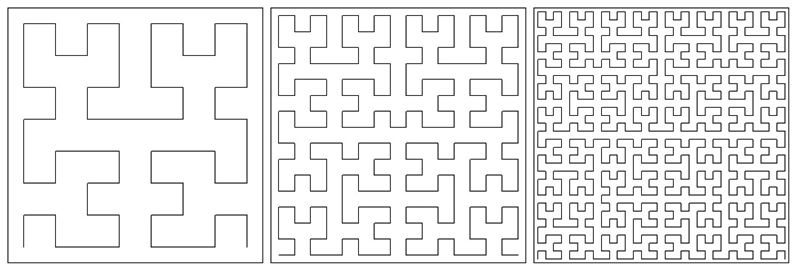
\includegraphics[width=\linewidth]{fig1}
  \caption{Examples of approximations of the Peano space-filling curves (the approximation density is equal to 2, 3 and 4 correspondingly)}
  \label{fig:1}
\end{figure}

Let $f(y)$ be the function to be minimized for which $k$, $k \geq 2$, optimization iterations are performed, and the search information $A_k$ from (\ref{eq:13}) is obtained. To adaptively select the points of the next iterations, the optimization algorithm has to evaluate the possibility of placing the global minimum in the subintervals, into which the interval [0,1] is divided by the points $x_i$, $1 \leq i \leq k$, of previously performed iterations of the global search. This assessment can be performed by introducing \textit{characteristics} of the subintervals, the value of which would be proportional to the degree to which the global minimum can be located in these subintervals
\begin{equation}\label{eq:15}
R(i)=\mathcal{R} (i,A_k ), 1 < i \leq k.
\end{equation}

The type of characteristics $R(i)$, $1 < i \leq k$, is a key design element of global optimization algorithms. For example, for an algorithm that builds a uniform dense grid in the search domain, the characteristics may simply be the length of the interval
\begin{equation}\label{eq:16}
R(i)=(x_i-x_{i-1}), 1 < i \leq k,
\end{equation}
where the points $x_i$, $1 < i \leq k$, are from $A_k$.

For the multidimensional generalizations of the algorithms proposed in \cite{c34,c35}, the characteristic is an estimate of the minimum possible value of the function being minimized on the interval, i.e.
\begin{equation}\label{eq:17}
R(i)=0.5 H \rho_i - 0.5 (z_{i-1} + z_i), \rho_i=(x_i - x_{i-1})^{1/N}, 1 < i \leq k,
\end{equation}
where the values $z_i$, $1<i \leq k$, are from $A_k$, $H$ is the H\"older constant from (\ref{eq:12}) for the reduced global optimization problem to be solved and $N$ is the dimensionality of the problem from (\ref{eq:1}). For the multidimensional generalized global search algorithm (GSA) \cite{c6,c23}, developed in the framework of the information-statistical approach, the characteristic has the form
\begin{equation}\label{eq:18}
R(i)=m \rho_i+\frac{(z_i-z_{i-1})^2}{m \rho_i }-2(z_{i-1}+z_i ), \rho_i=(x_i-x_{i-1})^{1/N}  ,1 < i \leq k,
\end{equation}
where $m$ is the numerical estimate of the H\"older constant obtained from the available search information $A_k$ from (\ref{eq:13})

\begin{equation}\label{eq:19}
m=r M, M=\max_{1 < i \leq k} \frac{|z_i-z_{i-1}|}{\rho_i}, \rho_i=(x_i-x_{i-1})^{1/N}  ,1 < i \leq k
\end{equation}
($r>1$ is the reliability parameter of the GSA algorithm).

A detailed description of the GSA algorithm is given in Algorithm \ref{alg:1} (see also \cite{c6}). The inputs of the algorithm are the function to be minimized $f(y)$\footnote{In the context of this paper, $f(y)$ can be regarded as one of the functions of the set $F(y)$ from (\ref{eq:3}).}, the search domain $D$ from (\ref{eq:2}), the reliability parameter $r > 1$, the required accuracy $\varepsilon > 0$ and the maximum permissible number of global search iterations $kmax$. The output of the algorithm is an estimate of the global minimum point $y_k^* =y(x_k^*)$, the value of the function to be minimized at this point $z_k^* =f(y_k^*)$  and the number of performed global search iterations $k$. In the course of calculations, the search information $A_k$\footnote{The set $A_k$ should be regarded as the search information $A_k(j)$ from (\ref{eq:13}) obtained by minimizing only one function $f(y)$.} from (\ref{eq:13}) is used, which contains the points of previously performed global search iterations $x_i$, $1 \leq i \leq k$, ordered in ascending order, and the values of the function to be minimized $z_i=f(y(x_i))$, $1\leq i \leq k$.

\begin{algorithm}[]
\caption{PSEUDO CODE OF THE GSA ALGORITHM} \label{alg:1}
\scriptsize
\hspace*{\algorithmicindent} \textbf{Input}: $f(y)$, $D$, $r$, $\varepsilon$, $K$;\\
\hspace*{\algorithmicindent} \textbf{Output}: $y_k^*$, $z_k^*$, $k$;
\begin{algorithmic}[1]
\State Initialize $A_2=\{(x_1=0,y_1=y(x_1 ),z_1=f(y(x_1 )),(x_2=1,y_2=y(x_2 ),z_2=f(y(x_2 ))\}$, $k = 2$, $stop = false$;
\While{$k < kmax$ \textbf{and not} $stop$} 
  \State Calculate the estimate of the H\"older constant $m$ from (\ref{eq:19}) using $A_k$;
  \State Calculate the interval characteristics $R(i)$ from (\ref{eq:18}) \textbf{for all} $i = 2, \dots, k$;
	\State Find the maximum characteristic 
	\begin{equation}\label{eq:20}
		R(t)=\max{R(i)}, 1 < i \leq k.
  \end{equation}
	\State Calculate the next iteration point
	\begin{equation}\label{eq:21}
	\begin{matrix}
	   x^{k+1}=\frac{x_t+x_{t-1}}{2}-sign(z_t-z_{t-1})(\frac{|z_t-z_{t-1}|}{m})^N/2r \\
		 sign(v)=\begin{cases}
		            1, &v>0,\\
		            0, &v=0,\\
								-1,&v<0
							\end{cases}
	\end{matrix}
	\end{equation}
	
	\State Check the stopping condition
	\begin{equation}\label{eq:22}
     stop = \begin{cases} true, &(x_t - x_{t-1})^{1/N} \leq \varepsilon,\\
		                      false,&(x_t - x_{t-1})^{1/N} > \varepsilon.
							\end{cases}		
  \end{equation}
  \If{ \textbf{not} $stop$}
	  \State Calculate $z^{k+1} = f( y(x^{k+1}))$;
    \State Insert $(x^{k+1}, y(x^{k+1}), z^{k+1})$ into the search information $A_k$;
    \State Increase $k = k + 1$;
  \EndIf
\EndWhile
\State Find the estimate of the global minimum point
\begin{equation}\label{eq:23}
y_k^*= y(x_l),  z_k^*=z_l,
\end{equation}
where $l= \argmin_{1 \leq i \leq k}z_i$.
\State \textbf{return} $y_k^*$, $z_k^*$, $k$;
\end{algorithmic}
\end{algorithm}

The sufficient condition for convergence of the GSA algorithm is the relation
\begin{equation}\label{eq:24}
m \geq 2H,
\end{equation}
that should be satisfied starting with some iteration of the global search. 

In the framework of the proposed approach, the GSA algorithm described above will be used to solve global optimization problems of the set $F$. Moreover, due to the informational connectivity (\ref{eq:5}) of the problems of the set $F$, the search information $A_k$ can be quickly transformed to the values of the next function to be minimized $f(y)$ of the set $F$ and GSA can minimize each successive function $f(y)$, taking into account the results of all previous calculations. The GSA algorithm for solving GO problems of the set $F$ and using search information $A_k$, will be referred to as the \textit{Multiple Global Search Algorithm} (MGSA).


\section{Parallel Computations for Solving Multiple Global Optimization Problems}\label{sec:4}

In keeping with the initial assumption that it is computationally expensive to calculate the values of the functions to be minimized of the set $F$ from (\ref{eq:3}), solving all global optimization problems (\ref{eq:1}) may require a huge amount of calculations, which increases with the number of problems to be solved. Thus, obtaining estimates of globally optimal decisions with reasonable time delays can only be achieved using parallel high-performance computational systems. 

An obvious way to apply parallel computing is to solve the problems of the set $F$ in parallel. Undoubtedly this approach is straightforward and does not require any additional efforts to be  implemented. In this case, if a sufficient number of computational devices ({cores/processors}) is available, the time needed to solve all problems from the set $F$ will be determined by the time used in solving the most time-consuming problem. However, this time may turn out to be quite long and necessitate the use of parallel computing to solve even one global optimization problem. However, well-known and widely used parallelization methods are poorly applicable in the case of global optimization problems. For example, the search domain distribution between processors for global optimization problems leads to the global minimum of the problems to be solved being located on only one of the processors, and all other processors will perform redundant calculations.

In the framework of the information-statistical theory, a general approach to parallelizing global optimization problems has been proposed -- parallel computing is provided by parallel (simultaneous) computing of the values of the minimized function at several different points in the search domain. This approach is general -- it can be applied to solving any global optimization problems in a parallel mode. And such an approach is efficient, since the most time consuming part of computations is parallelized due to the initial assumption that calculating the values of functions to be minimized is computationally expensive.

Next, we propose three different methods of applying this approach for parallel solutions to multiply global optimization problems (\ref{eq:1})-(\ref{eq:3}).

\subsection{Strategy 1: The Problem-oriented Parallel Scheme} \label{subsec:1}

In this method of parallel computing, it is proposed to solve the set $F$ of problems strictly sequentially, and to use all available computational resources only to solve just the optimization problem. When solving problems of the set $F$ sequentially, all available search information $A_k$, obtained in the calculation process is reused. 

To implement this approach, it is necessary to ensure that at each iteration of the global optimization problem, not one, but several points in the search domain $D$ are selected for parallel calculation of the values of the functions to be minimized at these points. In keeping with the fact that characteristically represented global search algorithms use the characteristics of the intervals $R(i)$, $1 < i \leq k$, from (\ref{eq:15}), to assess the possibility of locating the global minimum in the subintervals of the interval [0,1], it is most reasonable to select the points of the next iteration of the global search in the intervals with the maximum values of the characteristics \cite{c6}.

A parallel generalization of the MGSA algorithm (PMGSA-1) is given in Algorithm \ref{alg:2}.

Input data of this algorithm are the set of functions $F(y)$ from (\ref{eq:3}), the search domain $D$ from (\ref{eq:2}), the reliability parameter $r>1$, the required accuracy $\varepsilon > 0$, the maximum possible number of calculations of the values of the functions to be minimized $kmax$ and the number of available computational devices ({cores/processors}) with shared memory $q>1$. The results of executing the algorithm are the sets of estimates of global minimum points of the functions being minimized $Y$ and values of the functions $Z$ at these points, and the total number of executed iterations of global search $k$. As before, in the course of calculations we use the search information $A_k$, which contains the points of earlier iterations of global search $x_i$, $1 \leq i \leq k$, ordered in ascending order, and values of the current function being minimized $z_i=f(y(x_i))$, $1 \leq i \leq k$.

\begin{algorithm}[]
\caption{PSEUDO CODE OF THE PMGSA-1 ALGORITHM} \label{alg:2}
\scriptsize
\hspace*{\algorithmicindent} \textbf{Input}: $F(y)$, $D$, $r$, $\varepsilon$, $kmax$, $q$;\\
\hspace*{\algorithmicindent} \textbf{Output}: $Y$, $Z$, $k$;
\begin{algorithmic}[1]
\State Initialize $ k=2, A_2=\{(x_1=0,y_1=y(x_1),z_1=f(y(x_1)),(x_2=1,y_2=y(x_2),z_2=f(y(x_2))\} $;
\State $Y = \{\emptyset \}, Z = \{\emptyset\}$
\State Set $stop = false$;
\ForEach {$f(y)\subset \mathcal{F}(y)$ \textbf{and not} $stop$ }
\State Recalculate $A_k$ to the values of the function $f(y)$;
\While{$k < kmax$ \textbf{and not} $stop$} 
  \State Calculate the estimate of the H\"older constant $m$ from (\ref{eq:19}) using $A_k$;
  \State Calculate the interval characteristics $R(i)$ from (\ref{eq:18}) \textbf{for all} $i = 2, \dots, k$;
	\State Set $T = \{ \emptyset \}, XK = \{ \emptyset \}$;
	\ForEach { $i = 1..q$ } 
	// q is the number of available cores/processors
	  \State Find the interval with the maximum characteristic $t= \argmax_{1<i \leq k} R(i), i \notin T$;
		\State Calculate the iteration point $x^{k+i}$ in accordance with (\ref{eq:21});
    \State Insert $t$ in $T$ and $x^{k+i}$ in $XK$;

	\EndFor
  \State \textbf{for each} $t \in T$ \textbf{do if} $(x_t-x_{t-1} )^{1/N} \leq \varepsilon$ \textbf{then} $stop = true$;
	
	\If{ \textbf{not} $stop$}
	  \ForEach { $x \in XK $ } \textbf{in parallel}
	    \State Calculate $z = f( y(x))$;
      \State Insert $(x, y(x), z)$ into the search information $A_k$;
      \State Increase $k = k + 1$;
	  \EndFor
  \EndIf
	\State Find the estimate of the global minimum point of the current function $f(y)$ in accordance with (\ref{eq:23});
	\State Insert $y_k^*$ in $Y$ and $z_k^*$ in $Z$;
  \EndWhile
\EndFor
\State \textbf{return} $Y$, $Z$, $k$;
\end{algorithmic}
\end{algorithm}

Results of the numerical experiments show that this approach of parallelizing the MGSA algorithm allows one to obtain near-linear speedup using up to $2^N$ computational cores ($N$ is the dimensionality of the global optimization problems to be solved). An example of using PMGSA-1 is given in Fig. \ref{fig:2}. On the left in Fig. \ref{fig:2} the MGSA result is given (55 iterations), on the right the PMGSA-1 result is shown (30 iterations, i.e. the speedup is 1.8). PMGSA-1 uses 2 cores, iteration points selected by the cores are marked by the different lines.

\begin{figure}
  \centering
  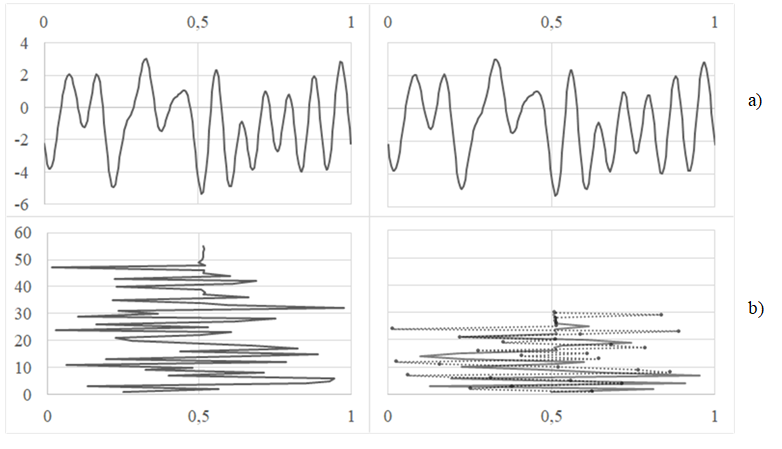
\includegraphics[width=\linewidth]{fig2}
  \caption{An example of using PMGSA-1 for solving the univariate optimization problem: a) the graph of the function being minimized, b) step-by-step selection of iteration points computed by the methods (the ordinate axis is the iteration number, the abscissa axis is the search domain)}
  \label{fig:2}
\end{figure}

\subsection{Strategy 2: The Competitive Parallel Scheme} \label{subsec:2}

Selecting several points at once for the same search iteration in the PMGSA-1 algorithm can result in redundant points compared to the sequential MGSA version, since these points are selected at the same state of search information $A_k$ from (\ref{eq:13}). Such an undesirable effect can be reduced by reducing the number of computational devices allocated to solve an optimization problem, while simultaneously increasing the number of parallel global optimization problems that are solved due to freed computational resources. In this case, the available computational resources can be distributed dynamically among problems in the global search process.

Assume, as before, that $q>1$ is the number of available computational devices (cores/processors) with shared memory, and $ns>1$ is the number of optimization problems\footnote{Without lost of generality, we will use sequential numbering of problems solved in parallel from 1 to $ns$.}  solved in parallel. Each optimization problem will compete for available computational resources -- the distribution of resources between problems can be carried out, as before, based on the values of interval characteristics. To calculate the characteristics, the problems solved in parallel have their own separate sets of search information $A_k (is)$, $1 \leq is \leq ns$, from (\ref{eq:13}), which match the set of iteration points $x_i$, $1 \leq i \leq k$, of the global search, but differ, accordingly, in the values $z_i (is)$, $1 \leq i \leq k$, of the minimized functions $f_{is} (y)$, $1 \leq is \leq ns$, from the set $F(y)$. As a result, in this case, to specify the intervals where the characteristics are computed, two indices $( is, t )$ are required, where $is$, $1 \leq is \leq ns$, is the number of the function to be minimized  $f_{is}(y)$ and  $t$, $1 \leq t \leq k$, is the number of the interval in the search information $A_k (is)$.

It should also be noted that when implementing this approach to compare the interval characteristics in different global optimization problems, the values of the function being minimized in the available search information should be normalized\footnote{After transformation (\ref{eq:25}), $z_k^*=0$ and $m_k=1$ are carried out for all $ns$ parallel problems.}
\begin{equation}\label{eq:25}
z(is)_i'=\frac{z(is)_i - z(is)_k^*}{m(is)_k}, 1 \leq i \leq k,1 \leq is \leq ns,
\end{equation}
where $z(is)_k^*$, $1 \leq is \leq ns$, are the estimates (\ref{eq:23}) of the minimum values of the functions being minimized, and $m(is)_k$, $1 \leq is \leq ns$, are the estimates (\ref{eq:19}) of the H\"older constants $H_{is}$, $1 \leq is \leq ns$, from (\ref{eq:12}). Further, when performing the steps of the algorithm, the converted values $z(is)_i'$, $1 \leq i \leq k$, $1 \leq is \leq ns$, should be used when calculating the characteristics of intervals and points of new iterations of the global search.

The new parallel version of the MGSA algorithm (the PMGSA-2 algorithm) obtained as a result of this approach is given in Algorithm \ref{alg:3}.

\begin{algorithm}[]
\caption{PSEUDO CODE OF THE PMGSA-2 ALGORITHM} \label{alg:3}
\scriptsize
\hspace*{\algorithmicindent} \textbf{Input}: $F(y)$, $D$, $r$, $\varepsilon$, $kmax$, $ns$;\\
\hspace*{\algorithmicindent} \textbf{Output}: $Y$, $Z$, $k$;
\begin{algorithmic}[1]
\State Initialize $ k=2, A_2=\{(x_1=0,y_1=y(x_1),z_1=f(y(x_1)),(x_2=1,y_2=y(x_2),z_2=f(y(x_2))\} $;
\State Set $stop = false$;
\While{$k < kmax$ \textbf{and not} $stop$}
  \ForEach { $is = 1..ns$ }
	  \State Calculate the estimate of the H\"older constant $m(is)_k$ from (\ref{eq:19}) using $A_k(is)$;
		\State Find the estimate of the global minimum value $z(is)_k^*$ of the function $f_{is}(y)$ in accordance with (\ref{eq:23});
		\State Set $A_k'(is)=A_k (is)$;
		\State Normalize the values $z(is)_i'$, $1 \leq i \leq k$, in $A_k'(is)$ in accordance with (\ref{eq:25});
		\State Set $m_k (is)=1$;
	\EndFor
	
	\State Set $T = \{ \emptyset \}, XK = \{ \emptyset \}$;
	\ForEach { $i = 1..q$ } 
	// q is the number of available cores/processors
	  \State Find the interval with the maximum characteristic using $A_k' (is)$
		\begin{equation*}
			R_{is} (t)= \argmax_{1 \leq is \leq ns, 1 < i \leq k} R(i),i \notin T;
	  \end{equation*}
		
		\State Calculate the iteration point $x^{k+i}$ using $A_k' (is)$ in accordance with (\ref{eq:21});
    \State Insert $t$ in $T$, $is$ in $IS$ and $x^{k+i}$ in $XK$;

	\EndFor
  \State \textbf{for each} $t \in T$ \textbf{do if} $(x_t-x_{t-1} )^{1/N} \leq \varepsilon$ \textbf{then} $stop = true$;
	
	\If{ \textbf{not} $stop$}
	  \ForEach { $x \in XK $ } \textbf{in parallel}
		  \State Take $is$ from $IS$;
	    \State Calculate $z = f_{is}(y(x))$;
      \State Insert $(x, y(x), z)$ into the search information $A_k$;
      \State Increase $k = k + 1$;
	  \EndFor
  \EndIf
	\EndWhile
	\State Set $Y = \{ \emptyset \}, Z = \{ \emptyset \}$;
	\ForEach { $iz = 1..ns$ }
	  \State Find the estimate of the global minimum point $y_k^*$ using $A_k (is)$ in accordance with (\ref{eq:23});
	  \State Insert $y_k^*$ in $Y$ and $z_k^*$ in $Z$;
	\EndFor

\State \textbf{return} $Y$, $Z$, $k$;
\end{algorithmic}
\end{algorithm}

Let us briefly explain the rules for performing a parallel iteration of the global search. The characteristics of the intervals are calculated for all $ns$ problems to be solved in parallel, and $q$ intervals with the maximum values of the characteristics are selected among them (lines 12-16). As a result, the available computational resources are distributed dynamically among problems -- computational devices can be distributed evenly between different problems, or they can be allocated to only one problem with the best interval characteristics. After calculating the values of the functions being minimized, the new search data obtained is added to the search information of all solved problems; regardless of where the intervals for iterating the global search were selected, the search information of all solved problems is updated with a full set of new search data (lines 19-24).

The maximum efficiency of the proposed PMGSA-2 algorithm is achieved if the global minimum in parallel problems is reached at the same point in the search domain. In any case, getting additional search information from simultaneously solved problems can significantly reduce the time needed to solve each global search problem. This conclusion is rather obvious if the global minima points of the functions $f_i (y)$, $1 \leq is \leq ns$, of the set $F$ from (\ref{eq:3}) are situated in the same small neighborhood of the search domain $D$ from (\ref{eq:2}). But even in the case when the global minima points of different functions differ much from each other, the values of different functions $f_i (y)$, $1 \leq is \leq ns$, of the set $F$ computed in the process of global search can be used for each function separately. Thus, in PMGSA-2 the execution of one parallel iteration using $q$ computational devices adds $q$ computation results. Increasing the amount of available search information allows adaptive global search algorithms to select points for the next iterations of the global search in a more reasonable manner. In the limiting case, when performing sufficiently many iterations $k \gg 1$, the amount of search information can be sufficient to find the global minimum point of the next problem in the set $F$ without any additional iterations. This effect is proved also by the results of numerical experiments in Section \ref{sec:5}. An example of how PMGSA-2 selects the intervals with the maximum characteristics is given in Fig.\ref{fig:3}.

\begin{figure}
  \centering
  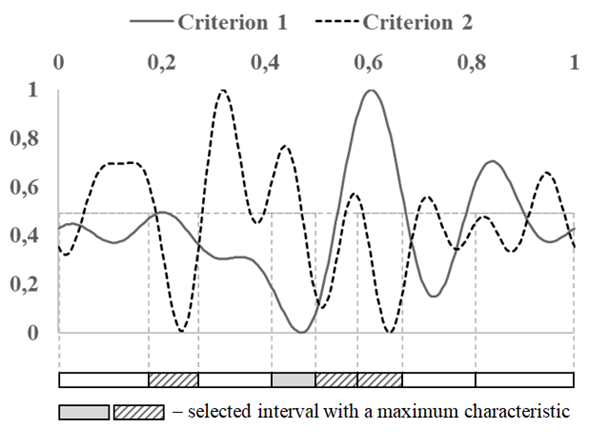
\includegraphics[width=0.7\linewidth]{fig3}
  \caption{An example of intervals selection by the PMGSA-2 algorithm}
  \label{fig:3}
\end{figure}

\subsection{Strategy 3: The Cooperative Parallel Scheme} \label{subsec:3}

When using computational devices with shared memory, the number of {cores/processors} is quite limited -- the number of cores on one computational node usually does not exceed 12-24. For increasing possible parallelism, it becomes inevitable to use a distributed memory computational system with several computational nodes.

Let $p>1$ be the number of computational devices with distributed memory, each of which has $q>1$ computational cores (that is, the total number of cores in a computational system is $p*q$). 

In the framework of the proposed approach, a parallel global optimization algorithm (the PMGAS-3 algorithm) is proposed for distributed memory computational systems, the main rules of which are as follows.


1) Solving the problems of the set $F(y)$ from (\ref{eq:3}) is carried out sequentially in groups; the number of problems in each group coincides with the number of available computational cores $p*q$.

2) Each computational node is applied for solving $q$ optimization problems using the PMGSA-2 algorithm.

3) At the end of each parallel iteration of the global search, the results of the iteration $(x^{k+j},z^{k+j} )$, $1 \leq j \leq q$, of each node are transferred to all available computational nodes with the necessary recalculation of the values of functions being minimized in accordance with the transformation $Z$ from (\ref{eq:5}).

4) Before performing a new iteration, each computational node accepts the search data transmitted to it and adds this data to the search information $A_k (is)$, $1\leq is \leq q$, from (\ref{eq:13}).
	
In this way, in keeping with the above rules, the PMGSA-3 algorithm is distributed -- the problems of the set $F(y)$ are solved independently on different computational nodes. During the global search process, computational nodes exchange the calculation results that are obtained; after each iteration of the global search, the search information for each problem being solved is updated with $p*q$ calculated values of the function being minimized. Thus, the more computational nodes there are (and accordingly, the problems that are solved simultaneously), the faster, as a rule, each optimization problem is solved. This is evidenced, in particular, by the results of numerical experiments that were performed (see Section \ref{sec:5}). An example of how PMGSA-3 performs an optimization iteration is given in Fig. \ref{fig:4}.

\begin{figure}
  \centering
  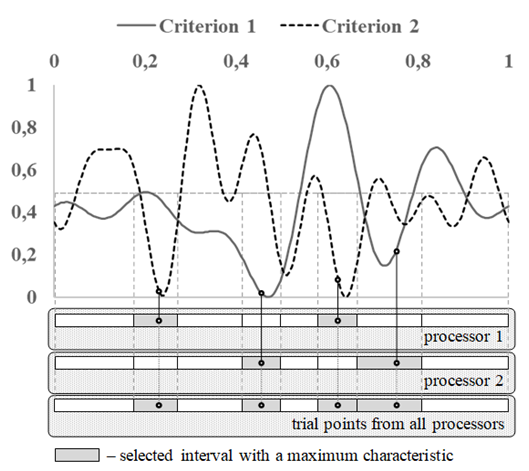
\includegraphics[width=0.7\linewidth]{fig4}
  \caption{Intervals and trial points selected by the PMGSA-3 algorithm}
  \label{fig:4}
\end{figure}

\section{Results of Numerical Experiments}\label{sec:5}

Numerical experiments were performed on the supercomputers Lobachevsky (University of Nizhni Novgorod) and Endeavour (Intel Cluster). The first supercomputer was used for optimization software system development. The numerical results were obtained by the second one with the following computational nodes: 2 Intel Xeon Platinum 8260L, 2.4 GHz, 256 GB RAM (i.e. a total of 48 CPU cores were available on each node). The executable program code was built by using the Intel Parallel Studio XE 2019 software package. The numerical experiments were performed using the Globalizer system \cite{c36}. This system offers an opportunity to solve computationally intensive multicriteria multiextremal optimization problems using the parallel global search algorithms presented in the paper.

First, we present the results achieved when comparing the MGSA algorithm with several multicriteria optimization algorithms \cite{c37}. In carrying out the experiments, the test two-criteria problem proposed in \cite{c38} was used:

\begin{equation}\label{eq:26}
f_1(y)=(y_1-1) y_2^2+1,f_2 (y)=y_2, 0 \leq y_1, y_2 \leq 1.
\end{equation}

This problem can be considered as an example of MGO, since, to approximate the Pareto set, the MGSA algorithm was applied for solving 50 subproblems $G (\lambda, y)$ from (\ref{eq:7}) for different values of convolution coefficients $\lambda$, uniformly distributed in the interval [0,1].



Solving the MCO problem is understood to mean the construction of a numerical approximation of the Pareto domain. To assess the quality of the approximation, the completeness and uniformity of coverage of the Pareto domain were compared using the following two indicators  \cite{c28,c37}:
\begin{itemize}
	 \item The hypervolume index (HV). This indicator characterizes how completely the Pareto domain is approximated (a higher value corresponds to a more complete coverage of the Pareto domain). 
	 \item The distribution uniformity index (DU). This indicator characterizes how uniformly the Pareto domain is covered (a lower value corresponds to a more uniform coverage of the Pareto domain).
\end{itemize}

During the experiments, five multicriteria optimization algorithms were compared: the Monte-Carlo (MC) method, the genetic algorithm SEMO from the PISA library \cite{c39}, the Non-uniform coverage (NUC) method \cite{c37}, the bi-objective Lipschitz optimization (BLO) method \cite{c38} and the MGSA algorithm. The results of solving the problem (\ref{eq:26}) for all these methods (except for MAGCS) were obtained in \cite{c38} -- see Table \ref{tab:1}.

\begin{table}[ht]
\centering
\caption{Comparison of the effectiveness of multicriteria optimization algorithms}
\label{tab:1}
\begin{tabular}{cccccc}
\hline
Method                                                                                     & MC    & SEMO  & NUC   & BLO   & \textbf{MGSA} \\ \hline
Iteration number                                          & 500   & 500   & 515   & 498   & \textbf{370}   \\
\begin{tabular}[c]{@{}c@{}}Number of Pareto optimal points\end{tabular} & 67    & 104   & 29    & 68    & \textbf{100}    \\
HV                                                        & 0.300 & 0.312 & 0.306 & 0.308 & \textbf{0.316} \\
DU                                                        & 1.277 & 1.116 & 0.210 & 0.175 & \textbf{0.101} \\ \hline
\end{tabular}
\end{table}

These numerical results show that the MGSA algorithm has a noticeable advantage in all performance indicators when compared with the methods of multicriteria optimization being considered, even when solving relatively simple MGO problems.

Further the numerical experiments were performed for evaluating the efficiency of the parallel PMGSA-1,2,3 algorithms in solving the MGO problems. In the experiments, the MGO problems were generated as problems seeking a set of efficient solutions to the MCO problems using the minimax convolution $G (\lambda, y)$ from (\ref{eq:7}) for different values of the convolution coefficients $\lambda$, uniformly distributed in the domain $\Lambda$. Given the original assumption about the high complexity of computing the values of functions being minimized of the set $F$ from (\ref{eq:3}), the efficiency of the proposed methods is evaluated by the number of optimization iterations performed by the methods to achieve the required accuracy under the stopping condition from (\ref{eq:22}).

In the first series of numerical experiments, five-criteria four-dimensional MCO problems were solved, i.e. $N = 4$, $m = 5$. In the experiments, 100 MCO problems were solved, in which multiextremal functions obtained by using the GKLS generator \cite{c40} were used as the efficiency criteria; for each problem 100 efficient solutions were calculated (i.e., a total of 10,000 subproblems $G (\lambda, y)$ were solved). The results obtained (the number of search iterations performed before the stopping condition was fulfilled) were averaged out over the number of MCO problems solved. In solving the problems, the search accuracy $\varepsilon = 0.05$ from (\ref{eq:22}) and the reliability parameter $r = 5.6$ from (\ref{eq:19}) were used. 

The results of the numerical experiments are presented in Table \ref{tab:2}. The first three rows of the Table contain information about the computational resources used during the experiments. The first row marked as ``$p$'' indicates the number of computational nodes used. The number of cores used within a single node is presented in the second row marked as ``$q$''. The total number of cores used is presented in the third row marked as ``$p*q$''. The rows four through six show the average number of iterations performed by PMGSA-1,2,3 for solving a single MCO problem (i.e., 100 GO problems) accordingly.

\begin{table}[ht]
\centering
\caption{The results of a series of experiments to solve five-criteria four-dimensional MCO problems}
\label{tab:2}
\begin{adjustbox}{max width=\textwidth}
\begin{tabular}{cccccccc}
\hline
\multicolumn{8}{c}{Computational resources used}                                                                                                                           \\ \hline
p                   & 1                     & 1                   & 1                  & 1                  & 2                  & 5                  & 10                 \\
q                   & 1                     & 5                   & 25                 & 48                 & 48                 & 48                 & 48                 \\
p*q                 & 1                     & 5                   & 25                 & 48                 & 96                 & 240                & 480                \\ \hline
\multicolumn{8}{c}{Average number of iterations for solving one   MCO problem}                                                                                             \\ \hline
PMGSA-1             & 117,490.8             & 19,586.9            & 4,232.4            & 2,116.5            & -                  & -                  & -                  \\
PMGSA-2             & 130,027.1             & 20,002.0            & 4,320.1            & 2,160.7            & -                  & -                  & -                  \\
PMGSA-3             & 117,490.8             & 19,586.9            & 4,232.4            & 2,116.5            & 1,064.6            & 534.3              & 285.5              \\ \hline
\multicolumn{8}{c}{Speedup obtained by using parallel methods}                                                                                                             \\ \hline
PMGSA-1             & 1                     & 6.0                 & 27.8               & 55.5               & -                  & -                  & -                  \\
PMGSA-2             & 1                     & 6.5                 & 30.1               & 60.2               & -                  & -                  & -                  \\
PMGSA-3             & 1                     & 6.0                 & 27.8               & 55.5               & 110.4              & 219.9              & 411.5              \\ \hline
\multicolumn{8}{c}{\begin{tabular}[c]{@{}c@{}}Overall reduction of executed iterations provided   \\ by parallel computations and reusing search information\end{tabular}} \\ \hline
PMGSA-1             & 11.9                  & 71.3                & 330.0              & 659.9              & -                  & -                  & -                  \\
PMGSA-2             & 10.7                  & 69.8                & 323.3              & 646.5              & -                  & -                  & -                  \\
PMGSA-3             & 11.9                  & 71.3                & 330.0              & 659.9              & 1,312.0            & 2,614.4            & 4,892.5            \\ \hline
\end{tabular}
\end{adjustbox}
\end{table}

It should be noted that for the initial sequential GSA algorithm without reusing search information, an average of 1,396,804.1 iterations are required to solve a single MCO problem. The overall reduction of the number of executed iterations, taking into account the effect of reusing search information, is indicated in the last three rows of Table \ref{tab:2}.

\begin{figure}
  \centering
  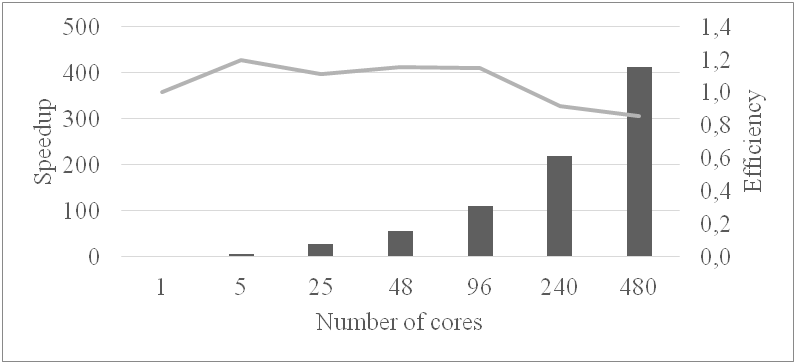
\includegraphics[width=0.7\linewidth]{fig5}
  \caption{Speedup and efficiency of the PMGSA-3 algorithm in solving five-criteria four-dimensional MCO problems}
  \label{fig:5}
\end{figure}


It follows from the results of the experiments (see also Fig. \ref{fig:5}), that the proposed parallel methods provide superlinear speedup\footnote{Superlinear speedup can be achieved due to the fact that the sets of iteration points that are selected when performing iterations of the global search by sequential and parallel algorithms are not identical (the search information of the methods may differ).} and high scalability (maintaining the efficiency of parallel computing with an increase in the number of computational cores used). When using a single computational node and all available computational cores for shared memory computational systems, the computational speedup exceeds 55 (with 48 computational cores in use). When using 10 computational nodes (480 cores) with distributed memory, the speedup becomes 411.5. Taking into account the effect of search information reuse, the overall reduction of the number of global optimization iterations is more than 4,890 times.

In the second series of the experiments, the problems being solved were made more complicated by increasing the dimensionality -- the five-criterion six-dimensional MCO problem was solved, i.e., $N = 6$, $m = 5$. For solving these problems the parallel PMGSA-3 method was applied. When performing the experiments, the accuracy $\varepsilon = 0.1$ and the reliability $r = 5.6$ were used. The results of the experiments are presented in Table \ref{tab:3}.

The first three rows of the Table, as before, present the number of computational nodes used, the number of cores per a node and the total number of computational cores. The last three rows correspond to the number of global search iterations performed, the speedup achieved, and the overall reduction of executed iterations, taking into account the reuse of information (the average number of iterations performed by the sequential GSA algorithm without the reuse of search information for solving one MCO problem is, on average, 3,131,284.8).

Based on the results of the experiments, it can be seen that when the dimensionality of the problem is increased, the efficiency of parallel computations using the PMGSA-3 algorithm also increases (when using 480 cores, the speedup is 472.9). Taking into account the effect of search information reuse, the number of global optimization iterations is reduced, in total, by more than 4,160 times.


\begin{table}[ht]
\centering
\caption{Results of numerical experiments to solve the five-criterion six-dimensional MCO problem using the parallel PMGSA-3 method}
\label{tab:3}
\begin{adjustbox}{max width=\textwidth}
\begin{tabular}{ccccccc}
\hline
\multicolumn{7}{c}{Computational resources used}                                                                                                  \\ \hline
p                                                                                & 1         & 1        & 1        & 1        & 5       & 10      \\
q                                                                                & 1         & 5        & 25       & 48       & 48      & 48      \\
p*q                                                                              & 1         & 5        & 25       & 48       & 240     & 480     \\ \hline
\multicolumn{7}{c}{Results of numerical experiments}                                                                                              \\ \hline
Iterations                                                                       & 364,713.2 & 97,387.5 & 19,791.0 & 11,294.0 & 1,561.2 & 771.2   \\
Speedup                                                                          & 1         & 3.7      & 18.4     & 32.3     & 233.6   & 472.9   \\
\begin{tabular}[c]{@{}c@{}}Overall reduction \\ of iteration number\end{tabular} & 8.6       & 32.2     & 159.6    & 277.5    & 2,025.6 & 4,160.1 \\ \hline
\end{tabular}
\end{adjustbox}
\end{table}

In order to demonstrate the efficiency of the proposed approach, a problem of vibration isolation for a system with several degrees of freedom consisting of an isolated base and an elastic body has been solved. In this problem it is assumed that the protected object can be represented as a multi-mass mechanical system consisting of several material points connected by vibration damping elements. As the criteria, the maximum deformation and maximum displacement of the object relative to the base were minimized \cite{c41}. The number of variable parameters is $N=3$. 

To construct an approximation of the Pareto set, 50 multiextremal functions $G (\lambda, y)$ from (\ref{eq:7}) were minimized for different values of the convolution coefficients $\lambda$, uniformly distributed in the domain $\Lambda$. When performing the experiments, the search accuracy $\varepsilon = 0.025$ and the reliability parameter $r = 3$ were used. The results of the experiments are presented in Table \ref{tab:4}.

\begin{table}[]
\centering
\caption{Results of numerical experiments to solve the applied problem}
\label{tab:4}
\begin{adjustbox}{max width=\textwidth}
\begin{tabular}{ccccccc}
\hline
Computational                     & p                     & 1       & 1      & 1       & 1       & 5       \\
resources                         & q                     & 1       & 1      & 48      & 48      & 48      \\
used                              & p*q                   & 1       & 1      & 48      & 48      & 240     \\ \hline
\multicolumn{2}{c}{Method}                                & GSA     & MGSA   & PMGSA-1 & PMGSA-2 & PMGSA-3 \\
\multicolumn{2}{c}{Iterations}                            & 703,802 & 13,120 & 403     & 237     & 116     \\
\multicolumn{2}{c}{HV}                                    & 1.46    & 1.45   & 1.38    & 1.88    & 1.39    \\
\multicolumn{2}{c}{DU}                                    & 501.03  & 499.43 & 500.46  & 498.73  & 500.39  \\
\multicolumn{2}{c}{Speedup}                               & -       & 1      & 32.6    & 55.4    & 113.1   \\
\multicolumn{2}{c}{\begin{tabular}[c]{@{}c@{}}Overall reduction \\ of iteration number\end{tabular}} & 1       & 53.6   & 1,746.4 & 2,969.6 & 6,067.3 \\ \hline
\end{tabular}
\end{adjustbox}
\end{table}

The results of the numerical experiments demonstrate that all methods have found the sufficient approximation of the Pareto domain. The lowest number of iterations performed the PMGSA-3 method. In Fig. \ref{fig:6}, the computed approximation of the Pareto domain obtained by the PMGSA-2 method is presented.

\begin{figure}
  \centering
  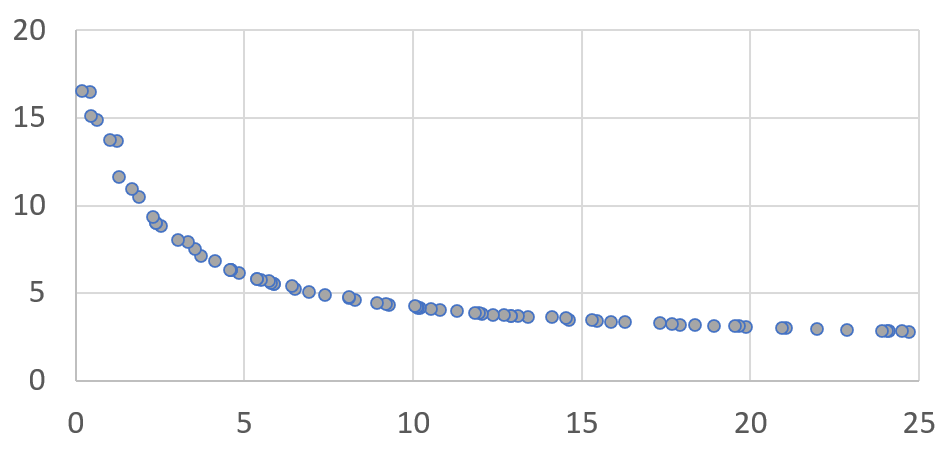
\includegraphics[width=0.7\linewidth]{fig6}
  \caption{Approximation of the Pareto domain for the problem of vibration isolation constructed by using PMAGS-2 method}
  \label{fig:6}
\end{figure}


\section{Conclusion}\label{sec:6}

The paper considers a new approach to solving multiple global optimization problems, in which minimized functions can be multiextremal, and calculating function values may require a huge amount of calculations. Problems of this kind are encountered, for example, when it is necessary to find several efficient solutions of multicriteria optimization problems or when part of the variable parameters of optimization problems can take only a number of discrete values. Problems of this class have a high computational complexity and the ability to solve such problems efficiently can be achieved only by using high-performance computational systems.

The proposed approach assumes that information connectivity exists in the global optimization problems being solved, when the calculated values of any function of the set of problems to be solved can be transformed to the values of any other functions without time consuming calculations. In such cases, all the search information obtained in solving a particular optimization problem can be used to solve all the other problems. Such reuse of search information can significantly reduce the amount of calculations performed, up to just a few iterations when solving the next problems of multiple global optimization.

The availability of informational connectivity significantly expands the possibilities of parallel solutions of the entire set of multiple global optimization problems. The paper proposes two parallel computational schemes: a cooperative scheme, which means the search information between the problems is exchanged between computational devices with distributed memory used for solving several GO problems in parallel, and a competitive scheme, which occurs when GO problems solved in parallel compete with each other for the use of available computational resources with shared memory.

Results of computational experiments show that the proposed approach allows us to significantly -- by tens and hundreds of times -- reduce the computational complexity of solving multiple global optimization problems.

In general, one can observe that the proposed approach is promising and requires further research. First, continued computational experiments must be carried out to solve the problems of multiple global optimization of varying computational complexity. It is also necessary to assess the possibility of using other global optimization algorithms within the framework of the proposed approach.

\section*{Acknowledgements} 
The work was supported by the Ministry of Science and Higher Education of the Russian Federation, agreement No 075-15-2020-808

\biboptions{sort&compress}
\bibliography{mybibfile}


\end{document}